%%
%% This is file `sample-acmsmall.tex',
%% generated with the docstrip utility.
%%
%% The original source files were:
%%
%% samples.dtx  (with options: `acmsmall')
%% 
%% IMPORTANT NOTICE:
%% 
%% For the copyright see the source file.
%% 
%% Any modified versions of this file must be renamed
%% with new filenames distinct from sample-acmsmall.tex.
%% 
%% For distribution of the original source see the terms
%% for copying and modification in the file samples.dtx.
%% 
%% This generated file may be distributed as long as the
%% original source files, as listed above, are part of the
%% same distribution. (The sources need not necessarily be
%% in the same archive or directory.)
%%
%% The first command in your LaTeX source must be the \documentclass command.
\documentclass[acmsmall]{acmart}

%%
%% \BibTeX command to typeset BibTeX logo in the docs
\AtBeginDocument{%
  \providecommand\BibTeX{{%
    \normalfont B\kern-0.5em{\scshape i\kern-0.25em b}\kern-0.8em\TeX}}}

\settopmatter{printacmref=false} % Removes citation information below abstract
\setcopyright{none}
\renewcommand\footnotetextcopyrightpermission[1]{} % removes footnote with conference information in first column
%\pagestyle{plain}

%% Rights management information.  This information is sent to you
%% when you complete the rights form.  These commands have SAMPLE
%% values in them; it is your responsibility as an author to replace
%% the commands and values with those provided to you when you
%% complete the rights form.
%\setcopyright{acmcopyright}
%\copyrightyear{2018}
%\acmYear{2018}
%\acmDOI{10.1145/1122445.1122456}


%%
%% These commands are for a JOURNAL article.
%\acmJournal{JACM}
%\acmVolume{37}
%\acmNumber{4}
%\acmArticle{111}
%\acmMonth{8}

%%
%% Submission ID.
%% Use this when submitting an article to a sponsored event. You'll
%% receive a unique submission ID from the organizers
%% of the event, and this ID should be used as the parameter to this command.
%%\acmSubmissionID{123-A56-BU3}

%%
%% The majority of ACM publications use numbered citations and
%% references.  The command \citestyle{authoryear} switches to the
%% "author year" style.
%%
%% If you are preparing content for an event
%% sponsored by ACM SIGGRAPH, you must use the "author year" style of
%% citations and references.
%% Uncommenting
%% the next command will enable that style.
%%\citestyle{acmauthoryear}
\usepackage{listings}
\usepackage{color}

\definecolor{dkgreen}{rgb}{0,0.6,0}
\definecolor{gray}{rgb}{0.5,0.5,0.5}
\definecolor{mauve}{rgb}{0.58,0,0.82}
\lstset{frame=tb,
	language=Java,
	aboveskip=3mm,
	belowskip=3mm,
	showstringspaces=false,
	columns=flexible,
	basicstyle={\small\ttfamily},
	numbers=none,
	numberstyle=\tiny\color{gray},
	keywordstyle=\color{blue},
	commentstyle=\color{dkgreen},
	stringstyle=\color{mauve},
	breaklines=true,
	breakatwhitespace=true,
	tabsize=3
}

%%
%% end of the preamble, start of the body of the document source.
\begin{document}

%%
%% The "title" command has an optional parameter,
%% allowing the author to define a "short title" to be used in page headers.
\title{Code Deobfuscation using Neural Program Learning Models}

%%
%% The "author" command and its associated commands are used to define
%% the authors and their affiliations.
%% Of note is the shared affiliation of the first two authors, and the
%% "authornote" and "authornotemark" commands
%% used to denote shared contribution to the research.
\author{Amin Fallahi}
\affiliation{%
	\institution{Syracuse University}
	\streetaddress{Center for Science and Technology, 111 College Pl}
	\city{Syracuse}
	\state{New York}
	%\country{USA}
}

%%
%% By default, the full list of authors will be used in the page
%% headers. Often, this list is too long, and will overlap
%% other information printed in the page headers. This command allows
%% the author to define a more concise list
%% of authors' names for this purpose.
\renewcommand{\shortauthors}{Fallahi, et al.}

%%
%% The abstract is a short summary of the work to be presented in the
%% article.
\begin{abstract}
	Code deobfuscation has gained attention in research for its wide applicability in forgery detection, privacy, and security. Several approaches have been proposed in past research that focus on identifier name recovery from a minified code or extracting information from obfuscated code. Most of them, use an statistical approach to deobfuscate code and get a good performance. In this research, we study neural networks and more specific neural program learning models on this task. We focus on Neural Turing Machine as a model that has been proven to work well on remembering information using its memory. We build the network using NTM, prepare an existing data set, and evaluate the network with various parameters against the data set.
\end{abstract}

%%
%% The code below is generated by the tool at http://dl.acm.org/ccs.cfm.
%% Please copy and paste the code instead of the example below.
%%
\begin{CCSXML}
<ccs2012>
 <concept>
  <concept_id>10010520.10010553.10010562</concept_id>
  <concept_desc>Computer systems organization~Embedded systems</concept_desc>
  <concept_significance>500</concept_significance>
 </concept>
 <concept>
  <concept_id>10010520.10010575.10010755</concept_id>
  <concept_desc>Computer systems organization~Redundancy</concept_desc>
  <concept_significance>300</concept_significance>
 </concept>
 <concept>
  <concept_id>10010520.10010553.10010554</concept_id>
  <concept_desc>Computer systems organization~Robotics</concept_desc>
  <concept_significance>100</concept_significance>
 </concept>
 <concept>
  <concept_id>10003033.10003083.10003095</concept_id>
  <concept_desc>Networks~Network reliability</concept_desc>
  <concept_significance>100</concept_significance>
 </concept>
</ccs2012>
\end{CCSXML}

\ccsdesc[500]{Computer systems organization~Embedded systems}
\ccsdesc[300]{Computer systems organization~Redundancy}
\ccsdesc{Computer systems organization~Robotics}
\ccsdesc[100]{Networks~Network reliability}

%%
%% Keywords. The author(s) should pick words that accurately describe
%% the work being presented. Separate the keywords with commas.
\keywords{datasets, neural networks, gaze detection, text tagging}


%%
%% This command processes the author and affiliation and title
%% information and builds the first part of the formatted document.
\maketitle

\section{Introduction}
One of the trending methods for improving software security and hiding program codes from users is code obfuscation. Some codes are meant to run on the browsers and are widely used to create dynamic content in web-pages. Many content providers try to hide the code from the user to improve their security and obscure the real function of code. Using a simple obfuscation technique, the providers make their program secure against attackers and are able to inject malicious code that can help advertisement, tracking the user, collecting user information, cross-site scripting attack, etc.

Obfuscation targets changing the code in a way that makes it hard for the human to understand what the code is actually doing by methods like changing variable/function names, altering execution order, loop unrolling, character encoding, etc. In contrast, code deobfuscation methods try to gain as much information from obfuscated codes and extract the program from unreadable code.

%Past research on code deobfuscation has achieved good accuracy for identifier recovery. But to our knowledge, 
Using an NPL model for solving this problem and how it performs can be an interesting study. NPL models use neural networks which are trained to learn and replicate code behavior, produce code from input/outputs, or complete previously written code. Code deobfuscation is an application that can be extended to a program learning task. Specifically, we can treat obfuscated identifier names as unknown holes in a program and try to recover them using an NPL model.

In this research, we use neural program learning methods to recover identifier (variables and functions) names from obfuscated program code. We study some currently used obfuscation and deobfuscation methods and how much identifier names the current approaches to deobfuscation can predict. Then, we use Neural Turing Machine as our program learning model and train it using available data sets. Finally, we evaluate our work and try to optimize the network by altering and tuning parameters to improve the performance.

The main contributions of this work are:
\begin{itemize}
	\item Application of neural program learning models on code deobfuscation task.
	\item Creating a neural activation data set usable in neural networks based on existing code data sets.
	\item Evaluating and comparing neural program learning models against traditional models and previous research for this task.
	\item Extending an existing Neural Turing Machine implementation[] to work with our model\footnote[1]{https://github.com/aminfallahi/Code-Deobfuscation-using-NTM}.
\end{itemize}

\textbf{Outline} In the remainder of this report, we discuss basic background knowledge required for studying this work in section 2. Then, we review and analyze the attacks which are possible to be launched against SGX enclave using side-channel information in section 3. In section 4, we introduce several defenses proposed by past research works, and in section 5 we analyze and compare the effectiveness of these defense methods in terms of security and performance. Finally, we conclude the research in section 6.

\section{Related Work}
Research on code deobfuscation has been a topic of interest during the recent years. Jiang et al. have proposed a method using Convolutional Neural Networks for detecting obfuscated JavaScript code \cite{jiangcnn}. Raychev et al. have developed a statistical model for recovering program properties (variable and function names) from obfuscated JavaScript code \cite{jsnice1} and have implemented a currently online website named JSNice \cite{jsnice3} which can predict the correct names for 63\% of identifiers from obfuscated code for their test data. They also have designed Nice2Predict \cite{nice2predict} which extracts statistical info out of obfuscated JavaScript code and is a base for JSNice. Raychev et al. also have done research on code completion and program synthesis \cite{Raychev2014} which is relevant to our problem. Bichsel et. al. have developed and tested a statistical method for deobfuscating Android applications \cite{bichselandroid} with 79.1\% success in recovering program identifier names. Another relevant research is \cite{forth} which studies filling program missing code slots using the behavior trained from the program input/output data. Lin et al. have done relevant research on translating natural language templates to program templates using Recurrent Neural Networks \cite{nlprnn}.

\section{Background}
\subsection{Neural Program Learning}
Neural program learning is the use of program behavior to train deep neural networks so they perform like the program or produce the code based on input/outputs, partial programs, etc. So, a neural network can be used as a programmer and also an interpreter. The research in this area has been proposed by several researchers during the past decade, varying from implementing logical gates using neural networks \cite{neto} to completing a partial program code \cite{forth}.
\subsection{Code Deobfuscation}
Obfuscation is a method used by programmers, specially in web services, to hide the running code from the user. When users visit a website using a browser with JavaScript enabled, several scripts will be executed in their browsers. The service providers, usually make the code unreadable by changing identifier names to meaningless tokens and then remove white space and tabs to decrease code size. Shrinking code size leads to less data transfer and faster page loading but changing identifier names is a method to hide the actual function of code from the user. Websites practice advertising, tracking, and other acts that are privacy concerns using these codes and keep their action secret by obfuscating the code.

Several methods have been proposed for deobfuscation. Basic methods recover tabs and spaces to make the code more readable but are not capable of recovering the actual code including identifier names. Some methods use machine learning and statistical approaches to recover identifier names. Also, some approaches target deciphering code that has been encrypted using different algorithms.

Listing 1. shows a piece of obfuscated JavaScript code grabbed from Facebook.com. This code is unminified using an online tool, Unminify \cite{unminify}, by inserting tabs and spaces for it to look more readable, but most of the identifier names are still obfuscated. As we can see most of them have been changed to single letter names, making it hard for anyone to understand what the code is actually doing.

Listing 2. shows the same code from Listing 1. deobfuscated using JSNice \cite{jsnice} tool which uses statistical methods to recover identifier names. As we can see, some of the identifier names have been recovered and the code is more understandable. However, we can not be sure how accurate are the names that are assigned to obfuscated identifiers.

\begin{lstlisting}[language=Java,caption={An obfuscated JavaScript code from facebook.com}]
__d("ContextualLayerAlignmentEnum", ["prop-types"], (function(a, b, c, d, e, f) {
	"use strict";
	a = {
		left: "left",
		center: "center",
		right: "right",
		propType: b("prop-types").oneOf(["left", "center", "right"]),
		values: ["left", "center", "right"]
	};
	e.exports = a
}), null);
\end{lstlisting}

\begin{lstlisting}[language=Java,caption={Deobfuscated JavaScript code from Listing 1. using JsNice\cite{jsnice} tool}]
'use strict';
__d("ContextualLayerAlignmentEnum", ["prop-types"], function(h, require, canCreateDiscussions, isSlidingUp, module, dontForceConstraints) {
	h = {
		left : "left",
		center : "center",
		right : "right",
		propType : require("prop-types").oneOf(["left", "center", "right"]),
		values : ["left", "center", "right"]
	};
	/** @type {(Object|string)} */
	module.exports = h;
}, null);
\end{lstlisting}




\subsection{Neural Turing Machine}
The idea behind Neural Turing Machines is to use an external memory to extend the capabilities of recurrent neural networks. The external memory and the network can then interact with attentional processes.

As shown in Fig. \ref{fig:ntmarch}, NTM is composed of two main components: the network controller and a memory bank which is basically a matrix used to store and retrieve information. In each time step, the network gets an input and produces an output. But NTM is also capable to perform read and write operations and alter the memory matrix. Like traditional Turing machines, NTM uses the term "head" to refer to a specific memory location.

\begin{figure}[h]
	\centering
	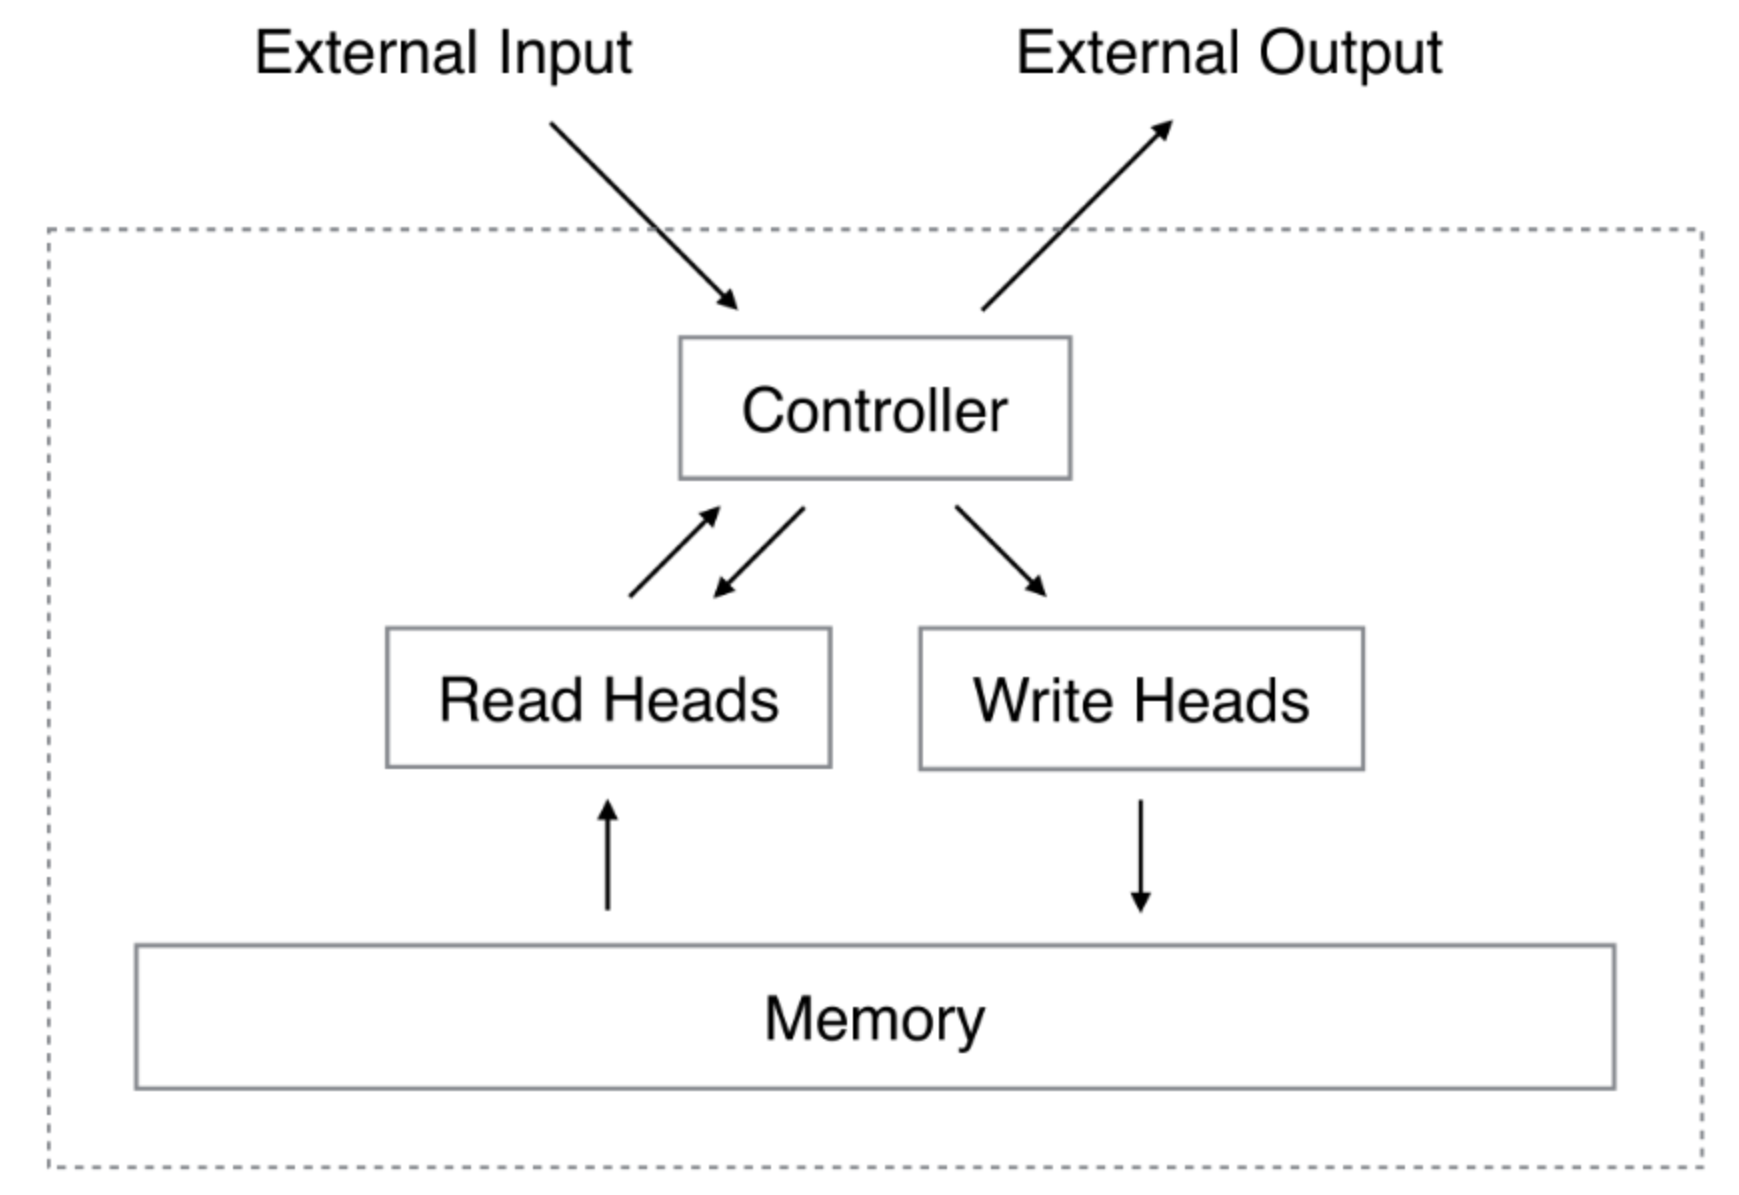
\includegraphics[scale=0.15]{figures/ntmarch}
	\caption{Neural Turing Machine architecture.}
	\Description{Neural Turing Machine architecture.}
	\label{fig:ntmarch}
\end{figure}

For network training it is preferred to use backpropagation and an optimizer like stochastic gradient decent (SGD) or Adam. For this purpose, NTM controller uses "blurry" reads and writes to interact with the memory, leading to the network being differentiable. That means, the controller uses a greater or lesser degree to read the whole memory instead of addressing and accessing each single element in memory. This is possible using an attention vector to focus on a part of memory and ignore the rest.

\subsubsection{Memory}
A memory $M_{t}$ is a $N \times M$ two dimensional matrix at time $t$, where $N$ indicates the number of memory locations, each storing a vector of size $M$.

\subsubsection{Read}
NTM uses a weighted sum of the memory for reading, where $w_t$ is a weight vector of size $N$ at time $t$:
\begin{equation}
r_t \longleftarrow \sum_{i} w_t(i)M_t(i)
\end{equation}

\subsubsection{Write}
A write operation is composed of an erase and an add operation. A vector $e_t$ of size $N$ is used for erasing and another vector $a_t$ is used for the add operation. Let $\tilde{M}_t$ be the intermediate memory after erase operation on $M_{t-1}$ and $1$ be a vector of ones:
\begin{equation}
\tilde{M_t}(i) \longleftarrow M_{t-1}(i)[1-w_t(i)e_t]
\end{equation}
Then, if both $w_t$ and $e_t$ at location $i$ are one, the memory location will reset to zero and if both are zero the memory will not be touched.

Finally, the add vector $a_t$ is used to perform the add operation on the intermediate memory state and produce the final memory matrix:
\begin{equation}
M_t(i) \longleftarrow \tilde{M}_t(i)+w_t(i)a_t
\end{equation}

\subsubsection{Addressing}
NTM produces the weighting vectors for read and write operations by combining content-based and location-based addressing mechanisms.

The content-based addressing compares a key vector $k_t$ with each $M_t(i)$ vector using cosine similarity measure and produces a normalized weight vector $w_t^c$ based on the similarity and a key strength vector $\beta_t$ which is used for increasing or decreasing focus precision:
\begin{equation}
w_t^c(i) \longleftarrow {{exp(\beta_t K[k_t, M_t(i)])} \over {\sum_{j} exp(\beta_t K[k_t,M_t(j)])}}
\end{equation}
Where using cosine similarity:
\begin{equation}
K[u,v] = {{u.v} \over {||u||.||v||}}
\end{equation}

For location-based addressing a scalar parameter $g_t \in (0,1)$ is introduced which is called interpolation gate and is used to mix $w_t^c$ and $w_{t-1}$ to produce the gated weighting $w_t^g$. This lets the controller know when to use which kind of memory addressing:
\begin{equation}
w_t^g \longleftarrow g_t w_t^c + (1-g_t)w_{t-1}
\end{equation}

NTM controller uses circular convolutional shift with all index arithmetic computed modulo $N$ with a shift vector $s_t$ to change the focus to another memory location and produce the shifted weight vector $\tilde{w}_t(i)$:
\begin{equation}
\tilde{w}_t(i) \longleftarrow \sum_{j=0}^{N-1} w_t^g(j)s_t(i-j)
\end{equation}

Finally, a scalar $\gamma$ is used for sharpening the final weighting and preventing it from blurring:
\begin{equation}
w_t(i) \longleftarrow {\tilde{w}_t(i)^{\gamma_t}} \over {\sum_{j} \tilde{w}_t(j)^{\gamma_t}}
\end{equation}

Figure \ref{fig:ntmaddressing} shows the flow of addressing mechanism.

\begin{figure}[h]
	\centering
	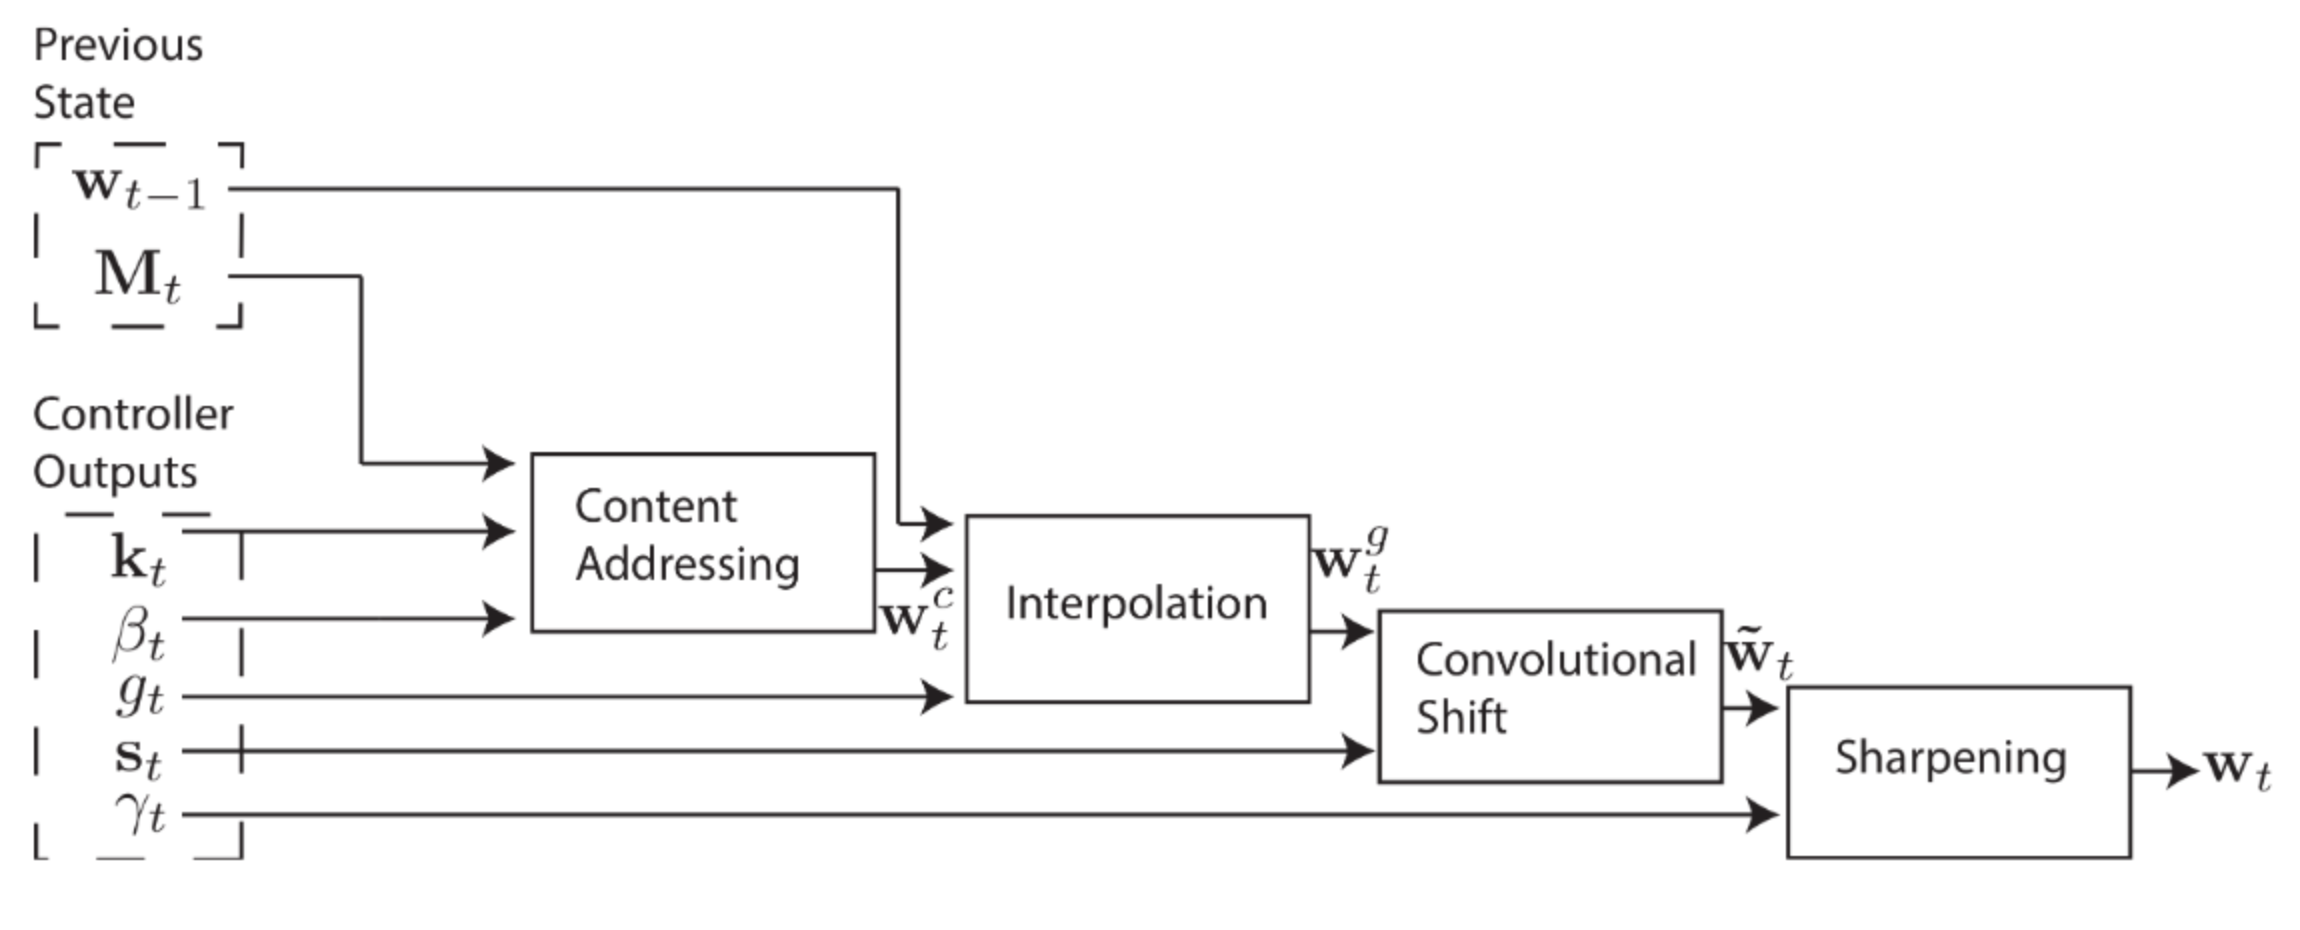
\includegraphics[scale=0.15]{figures/ntmaddressing}
	\caption{Flow diagram of Neural Turing Machine addressing mechanism.}
	\Description{Flow diagram of Neural Turing Machine addressing mechanism.}
	\label{fig:ntmaddressing}
\end{figure}

\section{Dataset Preparation}
Researchers in Secure, Reliable, and Intelligent Systems Lab at ETH Zurich have collected and published a data set of 150000 JavaScript programs and 150000 Python scripts as a part of their research \cite{jsnice} which is publicly available at \cite{bigcodedataset}. They have also parsed the programs and generated abstract syntax trees (AST) for all the programs in json format. In this research we build our dataset on top of their raw Python code dataset. For simplicity, we filter a set of 1848 programs each with less than 20 lines of code and smaller than 1 Kilobyte and truncate codes with unicode and non-ascii characters. Then, we use a simple Python tokenizer \cite{tokenizer} to extract all the tokens used in all programs. We sort the tokens and remove duplicates to create our final list containing 22973 tokens addressable with 15 binary bits. Afterwards, we create a list of vectors starting from 0b000000000000000 to 0b101100110111101 (22973) each representing one token. Finally, we use pyminify \cite{pyminify} (which is a simple tool for minifying Python codes) with --rename-globals option to rename all the variables to generate our obfuscated dataset and then we convert each program to a set of vectors based on their tokens and store the resulting dataset.

For our dataset to fit the NTM implementation we are using, we write a program to generate data batches. Each input sequence stores 128 token vectors and one vector of all ones indicating the end of sequence. The rest of sequence will be padded to 257 (2 times number of tokens minus 1 for the termination vector) vectors using vectors of all zeros. We also add one zero to all token vectors except the termination vector to differentiate them from it. So, the final shape of each input will be 257x16. Each output sequence stores 128 token vectors of 15 bits resulting in a shape of 128x15. The final batch that fits the NTM implementation we use is in the $[(sequence_length, array([[[]]], dtype=float32))]$ format and stores sequence length (128) and $n$ batches of inputs and outputs.
\section{Implementation}
The original authors of Neural Turing Machine have not published their source code to the public, but since 2014, multiple open source implementations have been released by various groups. Most of the implementations are limited and unstable. One the lates implementations which is more robust and reliable is the one by Collier et al. \cite{collier} which has won a best paper award. Therefore, we chose to modify their code to meet our application and use it for this research.

This implementation uses three tasks for evaluating neural turing machines: copy task that generates the same output by copying the input, repeat-copy task that extends copy task to copying input for specific number of times and produce it as output, associative recall that feeds a list of items to the network, queries one of them, and expects the next item in the list to be produced in output \cite{}.

We use copy task for our application. However, our data inputs and outputs are different and we are not using it for copying the input to output.

This implementation uses random sequences of vectors as the data. We implement a new data generator function to use our dataset instead of the randomly generated one. The details of our data generator is described in section 4.
\section{Evaluation}
\section{Discussion}
\section{Future Work}
\section{Conclusion}

\section{Template Overview}
As noted in the introduction, the ``\verb|acmart|'' document class can
be used to prepare many different kinds of documentation --- a
double-blind initial submission of a full-length technical paper, a
two-page SIGGRAPH Emerging Technologies abstract, a ``camera-ready''
journal article, a SIGCHI Extended Abstract, and more --- all by
selecting the appropriate {\itshape template style} and {\itshape
  template parameters}.

This document will explain the major features of the document
class. For further information, the {\itshape \LaTeX\ User's Guide} is
available from
\url{https://www.acm.org/publications/proceedings-template}.

\subsection{Template Styles}

The primary parameter given to the ``\verb|acmart|'' document class is
the {\itshape template style} which corresponds to the kind of publication
or SIG publishing the work. This parameter is enclosed in square
brackets and is a part of the {\verb|documentclass|} command:
\begin{verbatim}
  \documentclass[STYLE]{acmart}
\end{verbatim}

Journals use one of three template styles. All but three ACM journals
use the {\verb|acmsmall|} template style:
\begin{itemize}
\item {\verb|acmsmall|}: The default journal template style.
\item {\verb|acmlarge|}: Used by JOCCH and TAP.
\item {\verb|acmtog|}: Used by TOG.
\end{itemize}

The majority of conference proceedings documentation will use the {\verb|acmconf|} template style.
\begin{itemize}
\item {\verb|acmconf|}: The default proceedings template style.
\item{\verb|sigchi|}: Used for SIGCHI conference articles.
\item{\verb|sigchi-a|}: Used for SIGCHI ``Extended Abstract'' articles.
\item{\verb|sigplan|}: Used for SIGPLAN conference articles.
\end{itemize}

\subsection{Template Parameters}

In addition to specifying the {\itshape template style} to be used in
formatting your work, there are a number of {\itshape template parameters}
which modify some part of the applied template style. A complete list
of these parameters can be found in the {\itshape \LaTeX\ User's Guide.}

Frequently-used parameters, or combinations of parameters, include:
\begin{itemize}
\item {\verb|anonymous,review|}: Suitable for a ``double-blind''
  conference submission. Anonymizes the work and includes line
  numbers. Use with the \verb|\acmSubmissionID| command to print the
  submission's unique ID on each page of the work.
\item{\verb|authorversion|}: Produces a version of the work suitable
  for posting by the author.
\item{\verb|screen|}: Produces colored hyperlinks.
\end{itemize}

This document uses the following string as the first command in the
source file:
\verb|\documentclass[acmsmall]{acmart}|.

\section{Modifications}

Modifying the template --- including but not limited to: adjusting
margins, typeface sizes, line spacing, paragraph and list definitions,
and the use of the \verb|\vspace| command to manually adjust the
vertical spacing between elements of your work --- is not allowed.

{\bfseries Your document will be returned to you for revision if
  modifications are discovered.}

\section{Typefaces}

The ``\verb|acmart|'' document class requires the use of the
``Libertine'' typeface family. Your \TeX\ installation should include
this set of packages. Please do not substitute other typefaces. The
``\verb|lmodern|'' and ``\verb|ltimes|'' packages should not be used,
as they will override the built-in typeface families.

\section{Title Information}

The title of your work should use capital letters appropriately -
\url{https://capitalizemytitle.com/} has useful rules for
capitalization. Use the {\verb|title|} command to define the title of
your work. If your work has a subtitle, define it with the
{\verb|subtitle|} command.  Do not insert line breaks in your title.

If your title is lengthy, you must define a short version to be used
in the page headers, to prevent overlapping text. The \verb|title|
command has a ``short title'' parameter:
\begin{verbatim}
  \title[short title]{full title}
\end{verbatim}

\section{Authors and Affiliations}

Each author must be defined separately for accurate metadata
identification. Multiple authors may share one affiliation. Authors'
names should not be abbreviated; use full first names wherever
possible. Include authors' e-mail addresses whenever possible.

Grouping authors' names or e-mail addresses, or providing an ``e-mail
alias,'' as shown below, is not acceptable:
\begin{verbatim}
  \author{Brooke Aster, David Mehldau}
  \email{dave,judy,steve@university.edu}
  \email{firstname.lastname@phillips.org}
\end{verbatim}

The \verb|authornote| and \verb|authornotemark| commands allow a note
to apply to multiple authors --- for example, if the first two authors
of an article contributed equally to the work.

If your author list is lengthy, you must define a shortened version of
the list of authors to be used in the page headers, to prevent
overlapping text. The following command should be placed just after
the last \verb|\author{}| definition:
\begin{verbatim}
  \renewcommand{\shortauthors}{McCartney, et al.}
\end{verbatim}
Omitting this command will force the use of a concatenated list of all
of the authors' names, which may result in overlapping text in the
page headers.

The article template's documentation, available at
\url{https://www.acm.org/publications/proceedings-template}, has a
complete explanation of these commands and tips for their effective
use.

\section{Rights Information}

Authors of any work published by ACM will need to complete a rights
form. Depending on the kind of work, and the rights management choice
made by the author, this may be copyright transfer, permission,
license, or an OA (open access) agreement.

Regardless of the rights management choice, the author will receive a
copy of the completed rights form once it has been submitted. This
form contains \LaTeX\ commands that must be copied into the source
document. When the document source is compiled, these commands and
their parameters add formatted text to several areas of the final
document:
\begin{itemize}
\item the ``ACM Reference Format'' text on the first page.
\item the ``rights management'' text on the first page.
\item the conference information in the page header(s).
\end{itemize}

Rights information is unique to the work; if you are preparing several
works for an event, make sure to use the correct set of commands with
each of the works.

\section{CCS Concepts and User-Defined Keywords}

Two elements of the ``acmart'' document class provide powerful
taxonomic tools for you to help readers find your work in an online
search.

The ACM Computing Classification System ---
\url{https://www.acm.org/publications/class-2012} --- is a set of
classifiers and concepts that describe the computing
discipline. Authors can select entries from this classification
system, via \url{https://dl.acm.org/ccs/ccs.cfm}, and generate the
commands to be included in the \LaTeX\ source.

User-defined keywords are a comma-separated list of words and phrases
of the authors' choosing, providing a more flexible way of describing
the research being presented.

CCS concepts and user-defined keywords are required for all short- and
full-length articles, and optional for two-page abstracts.

\section{Sectioning Commands}

Your work should use standard \LaTeX\ sectioning commands:
\verb|section|, \verb|subsection|, \verb|subsubsection|, and
\verb|paragraph|. They should be numbered; do not remove the numbering
from the commands.

Simulating a sectioning command by setting the first word or words of
a paragraph in boldface or italicized text is {\bfseries not allowed.}

\section{Tables}

The ``\verb|acmart|'' document class includes the ``\verb|booktabs|''
package --- \url{https://ctan.org/pkg/booktabs} --- for preparing
high-quality tables.

Table captions are placed {\itshape above} the table.

Because tables cannot be split across pages, the best placement for
them is typically the top of the page nearest their initial cite.  To
ensure this proper ``floating'' placement of tables, use the
environment \textbf{table} to enclose the table's contents and the
table caption.  The contents of the table itself must go in the
\textbf{tabular} environment, to be aligned properly in rows and
columns, with the desired horizontal and vertical rules.  Again,
detailed instructions on \textbf{tabular} material are found in the
\textit{\LaTeX\ User's Guide}.

Immediately following this sentence is the point at which
Table~\ref{tab:freq} is included in the input file; compare the
placement of the table here with the table in the printed output of
this document.

\begin{table}
  \caption{Frequency of Special Characters}
  \label{tab:freq}
  \begin{tabular}{ccl}
    \toprule
    Non-English or Math&Frequency&Comments\\
    \midrule
    \O & 1 in 1,000& For Swedish names\\
    $\pi$ & 1 in 5& Common in math\\
    \$ & 4 in 5 & Used in business\\
    $\Psi^2_1$ & 1 in 40,000& Unexplained usage\\
  \bottomrule
\end{tabular}
\end{table}

To set a wider table, which takes up the whole width of the page's
live area, use the environment \textbf{table*} to enclose the table's
contents and the table caption.  As with a single-column table, this
wide table will ``float'' to a location deemed more
desirable. Immediately following this sentence is the point at which
Table~\ref{tab:commands} is included in the input file; again, it is
instructive to compare the placement of the table here with the table
in the printed output of this document.

\begin{table*}
  \caption{Some Typical Commands}
  \label{tab:commands}
  \begin{tabular}{ccl}
    \toprule
    Command &A Number & Comments\\
    \midrule
    \texttt{{\char'134}author} & 100& Author \\
    \texttt{{\char'134}table}& 300 & For tables\\
    \texttt{{\char'134}table*}& 400& For wider tables\\
    \bottomrule
  \end{tabular}
\end{table*}

\section{Math Equations}
You may want to display math equations in three distinct styles:
inline, numbered or non-numbered display.  Each of the three are
discussed in the next sections.

\subsection{Inline (In-text) Equations}
A formula that appears in the running text is called an inline or
in-text formula.  It is produced by the \textbf{math} environment,
which can be invoked with the usual
\texttt{{\char'134}begin\,\ldots{\char'134}end} construction or with
the short form \texttt{\$\,\ldots\$}. You can use any of the symbols
and structures, from $\alpha$ to $\omega$, available in
\LaTeX~\cite{Lamport:LaTeX}; this section will simply show a few
examples of in-text equations in context. Notice how this equation:
\begin{math}
  \lim_{n\rightarrow \infty}x=0
\end{math},
set here in in-line math style, looks slightly different when
set in display style.  (See next section).

\subsection{Display Equations}
A numbered display equation---one set off by vertical space from the
text and centered horizontally---is produced by the \textbf{equation}
environment. An unnumbered display equation is produced by the
\textbf{displaymath} environment.

Again, in either environment, you can use any of the symbols and
structures available in \LaTeX\@; this section will just give a couple
of examples of display equations in context.  First, consider the
equation, shown as an inline equation above:
\begin{equation}
  \lim_{n\rightarrow \infty}x=0
\end{equation}
Notice how it is formatted somewhat differently in
the \textbf{displaymath}
environment.  Now, we'll enter an unnumbered equation:
\begin{displaymath}
  \sum_{i=0}^{\infty} x + 1
\end{displaymath}
and follow it with another numbered equation:
\begin{equation}
  \sum_{i=0}^{\infty}x_i=\int_{0}^{\pi+2} f
\end{equation}
just to demonstrate \LaTeX's able handling of numbering.

\section{Figures}

The ``\verb|figure|'' environment should be used for figures. One or
more images can be placed within a figure. If your figure contains
third-party material, you must clearly identify it as such, as shown
in the example below.
\begin{figure}[h]
  \centering
  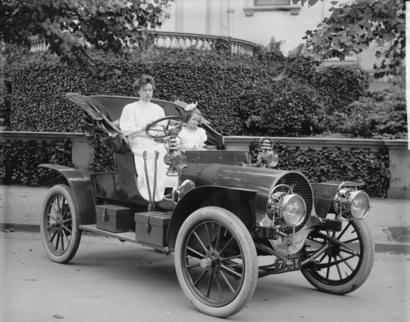
\includegraphics[width=\linewidth]{samples/sample-franklin}
  \caption{1907 Franklin Model D roadster. Photograph by Harris \&
    Ewing, Inc. [Public domain], via Wikimedia
    Commons. (\url{https://goo.gl/VLCRBB}).}
  \Description{The 1907 Franklin Model D roadster.}
\end{figure}

Your figures should contain a caption which describes the figure to
the reader. Figure captions go below the figure. Your figures should
{\bfseries also} include a description suitable for screen readers, to
assist the visually-challenged to better understand your work.

Figure captions are placed {\itshape below} the figure.

\subsection{The ``Teaser Figure''}

A ``teaser figure'' is an image, or set of images in one figure, that
are placed after all author and affiliation information, and before
the body of the article, spanning the page. If you wish to have such a
figure in your article, place the command immediately before the
\verb|\maketitle| command:
\begin{verbatim}
  \begin{teaserfigure}
    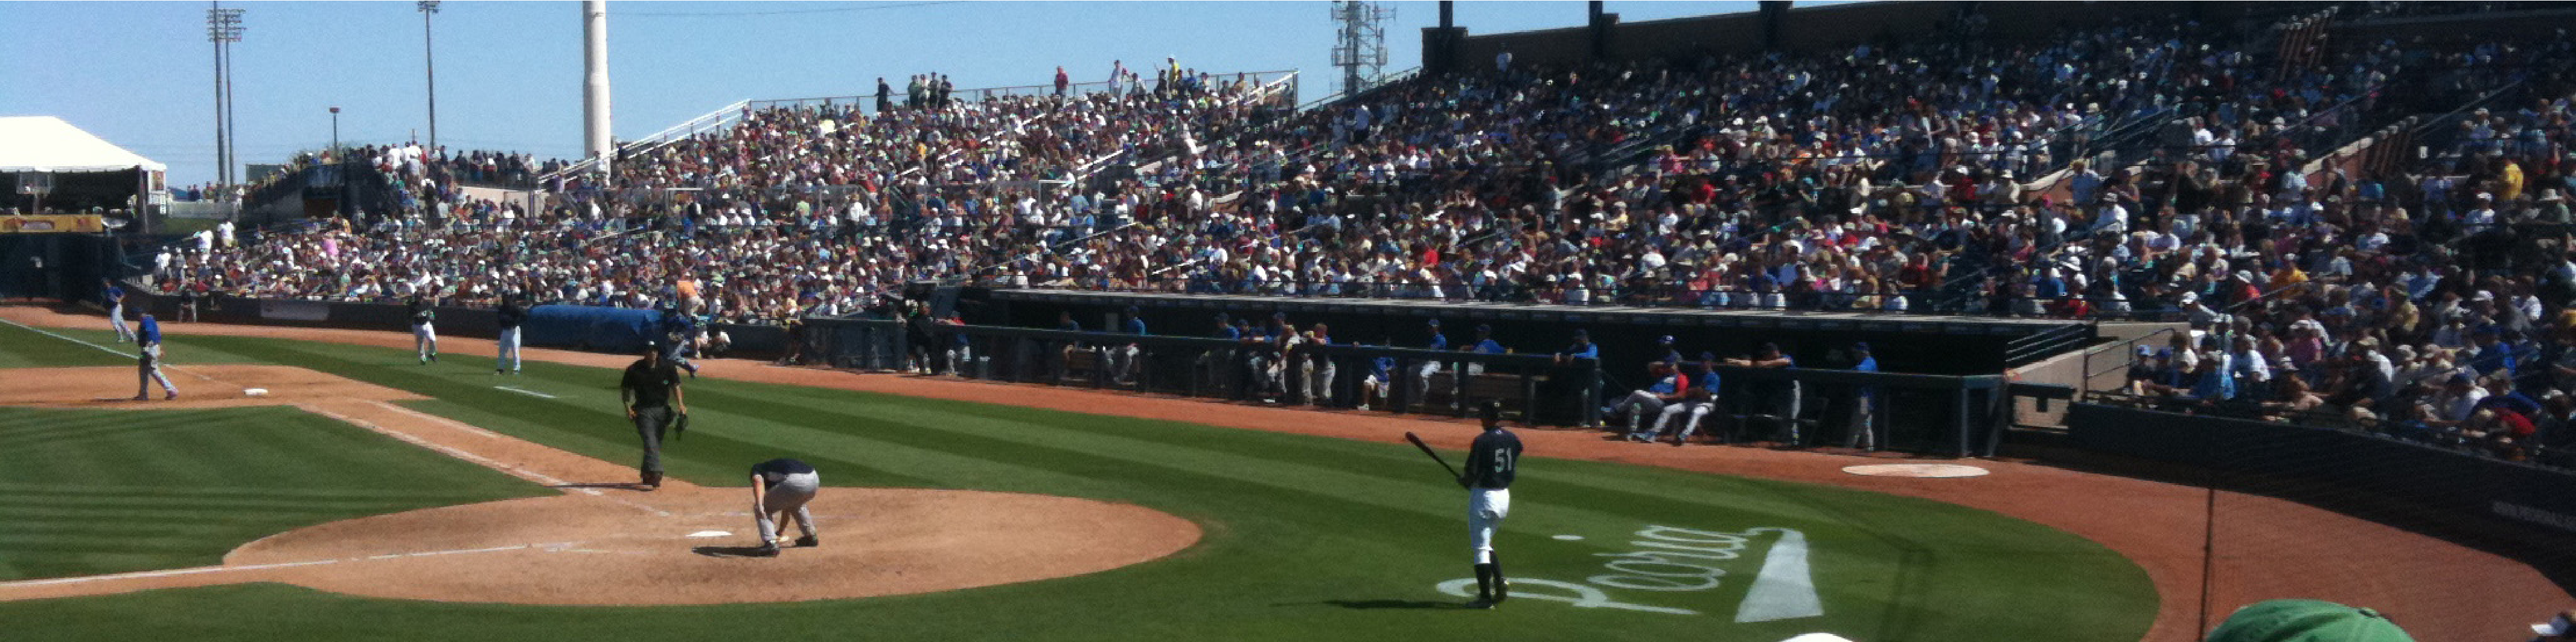
\includegraphics[width=\textwidth]{sampleteaser}
    \caption{figure caption}
    \Description{figure description}
  \end{teaserfigure}
\end{verbatim}

\section{Citations and Bibliographies}

The use of \BibTeX\ for the preparation and formatting of one's
references is strongly recommended. Authors' names should be complete
--- use full first names (``Donald E. Knuth'') not initials
(``D. E. Knuth'') --- and the salient identifying features of a
reference should be included: title, year, volume, number, pages,
article DOI, etc.

The bibliography is included in your source document with these two
commands, placed just before the \verb|\end{document}| command:
\begin{verbatim}
  \bibliographystyle{ACM-Reference-Format}
  \bibliography{bibfile}
\end{verbatim}
where ``\verb|bibfile|'' is the name, without the ``\verb|.bib|''
suffix, of the \BibTeX\ file.

Citations and references are numbered by default. A small number of
ACM publications have citations and references formatted in the
``author year'' style; for these exceptions, please include this
command in the {\bfseries preamble} (before
``\verb|\begin{document}|'') of your \LaTeX\ source:
\begin{verbatim}
  \citestyle{acmauthoryear}
\end{verbatim}

  Some examples.  A paginated journal article \cite{Abril07}, an
  enumerated journal article \cite{Cohen07}, a reference to an entire
  issue \cite{JCohen96}, a monograph (whole book) \cite{Kosiur01}, a
  monograph/whole book in a series (see 2a in spec. document)
  \cite{Harel79}, a divisible-book such as an anthology or compilation
  \cite{Editor00} followed by the same example, however we only output
  the series if the volume number is given \cite{Editor00a} (so
  Editor00a's series should NOT be present since it has no vol. no.),
  a chapter in a divisible book \cite{Spector90}, a chapter in a
  divisible book in a series \cite{Douglass98}, a multi-volume work as
  book \cite{Knuth97}, an article in a proceedings (of a conference,
  symposium, workshop for example) (paginated proceedings article)
  \cite{Andler79}, a proceedings article with all possible elements
  \cite{Smith10}, an example of an enumerated proceedings article
  \cite{VanGundy07}, an informally published work \cite{Harel78}, a
  doctoral dissertation \cite{Clarkson85}, a master's thesis:
  \cite{anisi03}, an online document / world wide web resource
  \cite{Thornburg01, Ablamowicz07, Poker06}, a video game (Case 1)
  \cite{Obama08} and (Case 2) \cite{Novak03} and \cite{Lee05} and
  (Case 3) a patent \cite{JoeScientist001}, work accepted for
  publication \cite{rous08}, 'YYYYb'-test for prolific author
  \cite{SaeediMEJ10} and \cite{SaeediJETC10}. Other cites might
  contain 'duplicate' DOI and URLs (some SIAM articles)
  \cite{Kirschmer:2010:AEI:1958016.1958018}. Boris / Barbara Beeton:
  multi-volume works as books \cite{MR781536} and \cite{MR781537}. A
  couple of citations with DOIs:
  \cite{2004:ITE:1009386.1010128,Kirschmer:2010:AEI:1958016.1958018}. Online
  citations: \cite{TUGInstmem, Thornburg01, CTANacmart}.

\section{Acknowledgments}

Identification of funding sources and other support, and thanks to
individuals and groups that assisted in the research and the
preparation of the work should be included in an acknowledgment
section, which is placed just before the reference section in your
document.

This section has a special environment:
\begin{verbatim}
  \begin{acks}
  ...
  \end{acks}
\end{verbatim}
so that the information contained therein can be more easily collected
during the article metadata extraction phase, and to ensure
consistency in the spelling of the section heading.

Authors should not prepare this section as a numbered or unnumbered {\verb|\section|}; please use the ``{\verb|acks|}'' environment.

\section{Appendices}

If your work needs an appendix, add it before the
``\verb|\end{document}|'' command at the conclusion of your source
document.

Start the appendix with the ``\verb|appendix|'' command:
\begin{verbatim}
  \appendix
\end{verbatim}
and note that in the appendix, sections are lettered, not
numbered. This document has two appendices, demonstrating the section
and subsection identification method.

\section{SIGCHI Extended Abstracts}

The ``\verb|sigchi-a|'' template style (available only in \LaTeX\ and
not in Word) produces a landscape-orientation formatted article, with
a wide left margin. Three environments are available for use with the
``\verb|sigchi-a|'' template style, and produce formatted output in
the margin:
\begin{itemize}
\item {\verb|sidebar|}:  Place formatted text in the margin.
\item {\verb|marginfigure|}: Place a figure in the margin.
\item {\verb|margintable|}: Place a table in the margin.
\end{itemize}

%%
%% The acknowledgments section is defined using the "acks" environment
%% (and NOT an unnumbered section). This ensures the proper
%% identification of the section in the article metadata, and the
%% consistent spelling of the heading.
\begin{acks}
To Robert, for the bagels and explaining CMYK and color spaces.
\end{acks}

%%
%% The next two lines define the bibliography style to be used, and
%% the bibliography file.
\bibliographystyle{ACM-Reference-Format}
\bibliography{sample-base}

%%
%% If your work has an appendix, this is the place to put it.
\appendix

\section{Research Methods}

\subsection{Part One}

Lorem ipsum dolor sit amet, consectetur adipiscing elit. Morbi
malesuada, quam in pulvinar varius, metus nunc fermentum urna, id
sollicitudin purus odio sit amet enim. Aliquam ullamcorper eu ipsum
vel mollis. Curabitur quis dictum nisl. Phasellus vel semper risus, et
lacinia dolor. Integer ultricies commodo sem nec semper.

\subsection{Part Two}

Etiam commodo feugiat nisl pulvinar pellentesque. Etiam auctor sodales
ligula, non varius nibh pulvinar semper. Suspendisse nec lectus non
ipsum convallis congue hendrerit vitae sapien. Donec at laoreet
eros. Vivamus non purus placerat, scelerisque diam eu, cursus
ante. Etiam aliquam tortor auctor efficitur mattis.

\section{Online Resources}

Nam id fermentum dui. Suspendisse sagittis tortor a nulla mollis, in
pulvinar ex pretium. Sed interdum orci quis metus euismod, et sagittis
enim maximus. Vestibulum gravida massa ut felis suscipit
congue. Quisque mattis elit a risus ultrices commodo venenatis eget
dui. Etiam sagittis eleifend elementum.

Nam interdum magna at lectus dignissim, ac dignissim lorem
rhoncus. Maecenas eu arcu ac neque placerat aliquam. Nunc pulvinar
massa et mattis lacinia.

\end{document}
\endinput
%%
%% End of file `sample-acmsmall.tex'.
__d("ViewportTrackingHooks", ["Base64"], (function(a, b, c, d, e, f) {
	__p && __p();
	var g = {},
	h = [];
	a = {
		registerFeedObject: function(a, c) {
			g[a] = b("Base64").encode(c)
		},
		updateVisibleViewportObjects: function(a) {
			var b = [],
			c = !1;
			for (var d = 0; d < a.length; d++) {
				var e = a[d],
				f = e.id;
				while (!(f in g) && e.firstChild != void 0 && e.firstChild.id != void 0 && e.firstChild.id.startsWith("u_")) f = e.firstChild.id, e = e.firstChild;
				f in g && (b.push(g[f]), (!(d in h) || h[d] != g[f]) && (c = !0))
			}!c && h.length != b.length && (c = !0);
			c && (h = b, typeof __EXT__updateVisibleViewportObjects === "function" && __EXT__updateVisibleViewportObjects(h))
		}
	};
	e.exports = a
}), null);
\end{lstlisting}
\begin{lstlisting}
'use strict';
__d("ViewportTrackingHooks", ["Base64"], function(__WEBPACK_EXTERNAL_MODULE_61__, require, canCreateDiscussions, isSlidingUp, module, dontForceConstraints) {
if (__p) {
__p();
}
var obj = {};
/** @type {!Array} */
var a = [];
__WEBPACK_EXTERNAL_MODULE_61__ = {
registerFeedObject : function(table, data) {
obj[table] = require("Base64").encode(data);
},
updateVisibleViewportObjects : function(queryEvents) {
/** @type {!Array} */
var b = [];
/** @type {boolean} */
var c = false;
/** @type {number} */
var i = 0;
for (; i < queryEvents.length; i++) {
var e = queryEvents[i];
var key = e.id;
for (; !(key in obj) && e.firstChild != void 0 && e.firstChild.id != void 0 && e.firstChild.id.startsWith("u_");) {
key = e.firstChild.id;
e = e.firstChild;
}
if (key in obj) {
b.push(obj[key]);
if (!(i in a) || a[i] != obj[key]) {
/** @type {boolean} */
c = true;
}
}
}
if (!c && a.length != b.length) {
/** @type {boolean} */
c = true;
}
if (c) {
/** @type {!Array} */
a = b;
if (typeof __EXT__updateVisibleViewportObjects === "function") {
__EXT__updateVisibleViewportObjects(a);
}
}
}
};
/** @type {(Object|string)} */
module.exports = __WEBPACK_EXTERNAL_MODULE_61__;
}, null);
\end{lstlisting}